\documentclass[svgnames,
               hyperref={colorlinks,citecolor=DeepPink4,linkcolor=FireBrick,urlcolor=Maroon},
               usepdftitle=false]  % see \hypersetup{} below
               {beamer}

\mode<presentation>{
  \usetheme{Madrid}
  %\usecolortheme{seagull}
  \usecolortheme{seagull}
  \setbeamercovered{transparent}
  \setbeamerfont{frametitle}{size=\large}
}

\setbeamercolor*{block title}{bg=red!10}
\setbeamercolor*{block body}{bg=red!5}

%\usepackage[svgnames]{xcolor}
\usepackage{hyperref}
\hypersetup{
    pdftitle = {Toward nonlinear multigrid for nonlinear variational inequalities},
    pdfauthor = {Ed Bueler},
    pdfsubject = {},
    pdfkeywords = {}
}

\usepackage[english]{babel}
\usepackage[latin1]{inputenc}
\usepackage{times}
\usepackage[T1]{fontenc}
\usepackage{empheq,bm,xspace,fancyvrb,soul}
\usepackage{tikz}
\usetikzlibrary{shapes,arrows.meta,decorations.markings,decorations.pathreplacing,fadings,positioning}
\usepackage[kw]{pseudo}
\pseudoset{left-margin=15mm,topsep=5mm,idfont=\texttt,st-left=,st-right=}

\newcommand{\eps}{\epsilon}
\newcommand{\RR}{\mathbb{R}}

\newcommand{\grad}{\nabla}
\newcommand{\Div}{\nabla\cdot}
\newcommand{\trace}{\operatorname{tr}}

\newcommand{\hbn}{\hat{\mathbf{n}}}

\newcommand{\bb}{\mathbf{b}}
\newcommand{\be}{\mathbf{e}}
\newcommand{\bbf}{\mathbf{f}}
\newcommand{\bg}{\mathbf{g}}
\newcommand{\bn}{\mathbf{n}}
\newcommand{\br}{\mathbf{r}}
\newcommand{\bu}{\mathbf{u}}
\newcommand{\bv}{\mathbf{v}}
\newcommand{\bw}{\mathbf{w}}
\newcommand{\bx}{\mathbf{x}}

\newcommand{\bF}{\mathbf{F}}
\newcommand{\bQ}{\mathbf{Q}}
\newcommand{\bU}{\mathbf{U}}
\newcommand{\bV}{\mathbf{V}}
\newcommand{\bX}{\mathbf{X}}

\newcommand{\btau}{\bm{\tau}}
\newcommand{\bxi}{\bm{\xi}}

\newcommand{\bzero}{\bm{0}}

\newcommand{\rhoi}{\rho_{\text{i}}}

\newcommand{\ip}[2]{\left(#1,#2\right)}

\newcommand{\mR}{R^{\bm{\oplus}}}
\newcommand{\iR}{R^{\bullet}}

\newcommand{\nn}{{\text{n}}}
\newcommand{\pp}{{\text{p}}}
\newcommand{\qq}{{\text{q}}}
\newcommand{\rr}{{\text{r}}}

\newcommand{\bus}{\bu|_s}
\newcommand{\oo}[1]{\displaystyle O\left(#1\right)}
\newcommand{\sold}{s_{\text{o}}}


\title[Multigrid for nonlinear VI]{Toward nonlinear multigrid \\ for nonlinear variational inequalities}

%\subtitle{\emph{x}}

\author{Ed Bueler}

\institute[UAF]{University of Alaska Fairbanks}

\date[]{February 2023}

%\titlegraphic{\begin{picture}(0,0)
%    \put(0,180){\makebox(0,0)[rt]{\includegraphics[width=4cm]{figs/software.png}}}
%  \end{picture}
%}

\titlegraphic{\hfill 
\includegraphics[width=0.15\textwidth]{images/uafbw.png}}

%% to start section counter at 0 see
%% https://tex.stackexchange.com/questions/170222/change-the-numbering-in-beamers-table-of-content


\begin{document}
\beamertemplatenavigationsymbolsempty

%\begin{frame}
%  \maketitle
%\end{frame}

{
  %\usebackgroundtemplate{\includegraphics[width=\paperwidth]{images/gray-british-clark2022.png}}
  \begin{frame}
    \titlepage
  \end{frame}
}

\begin{frame}{Outline}
  \tableofcontents[hideallsubsections]
\end{frame}


\section{variational inequalities (VIs) and obstacle problems}

\begin{frame}{the classical obstacle problem}

\begin{center}
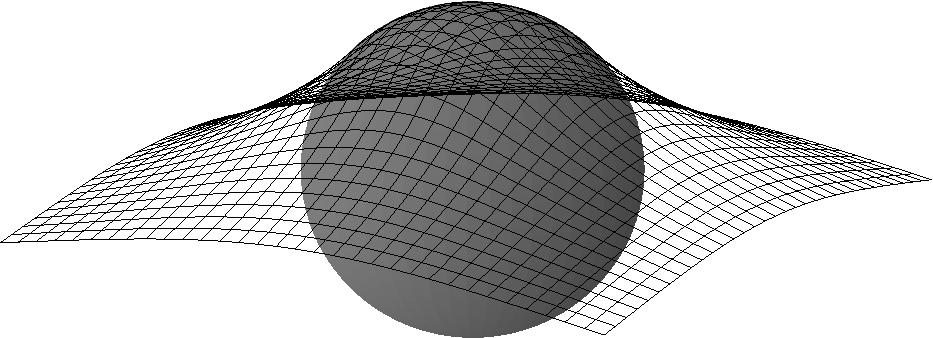
\includegraphics[width=0.6\textwidth]{images/obstacle65.pdf}
\end{center}

\begin{itemize}
\item x
\end{itemize}
\end{frame}

\begin{frame}{active sets, free boundaries}

\begin{columns}
\begin{column}{0.6\textwidth}
\begin{itemize}
\item x
\end{itemize}
\end{column}
\begin{column}{0.4\textwidth}
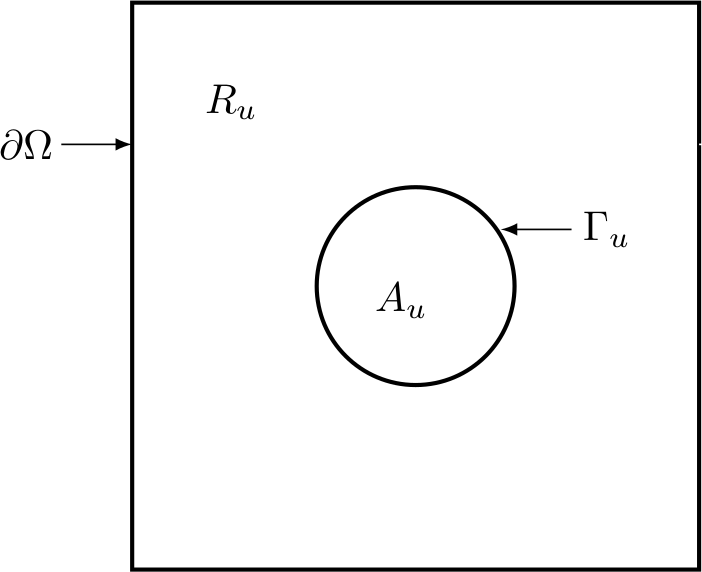
\includegraphics[width=0.6\textwidth]{images/obstacle-sets.png}
\end{column}
\end{columns}
\end{frame}


\begin{frame}{Newton iterations for VIs}

\begin{columns}
\begin{column}{0.6\textwidth}
\begin{itemize}
\item x
\end{itemize}
\end{column}
\begin{column}{0.4\textwidth}
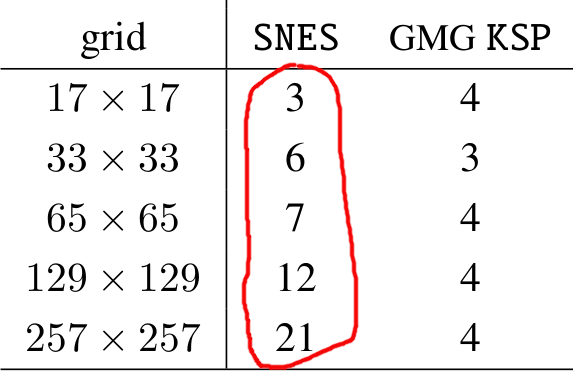
\includegraphics[width=\textwidth]{images/vi-newton-gmg-bad.png}

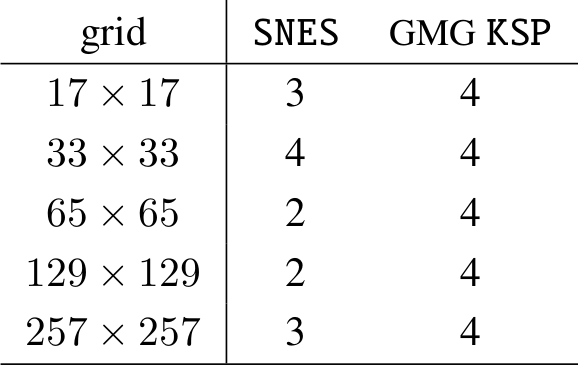
\includegraphics[width=\textwidth]{images/vi-newton-gmg-good.png}
\end{column}
\end{columns}
\end{frame}


\begin{frame}{Newton-multigrid for VIs}

xxx
\end{frame}


\begin{frame}{optimality}

\begin{columns}
\begin{column}{0.6\textwidth}
\begin{itemize}
\item x
\end{itemize}
\end{column}
\begin{column}{0.4\textwidth}
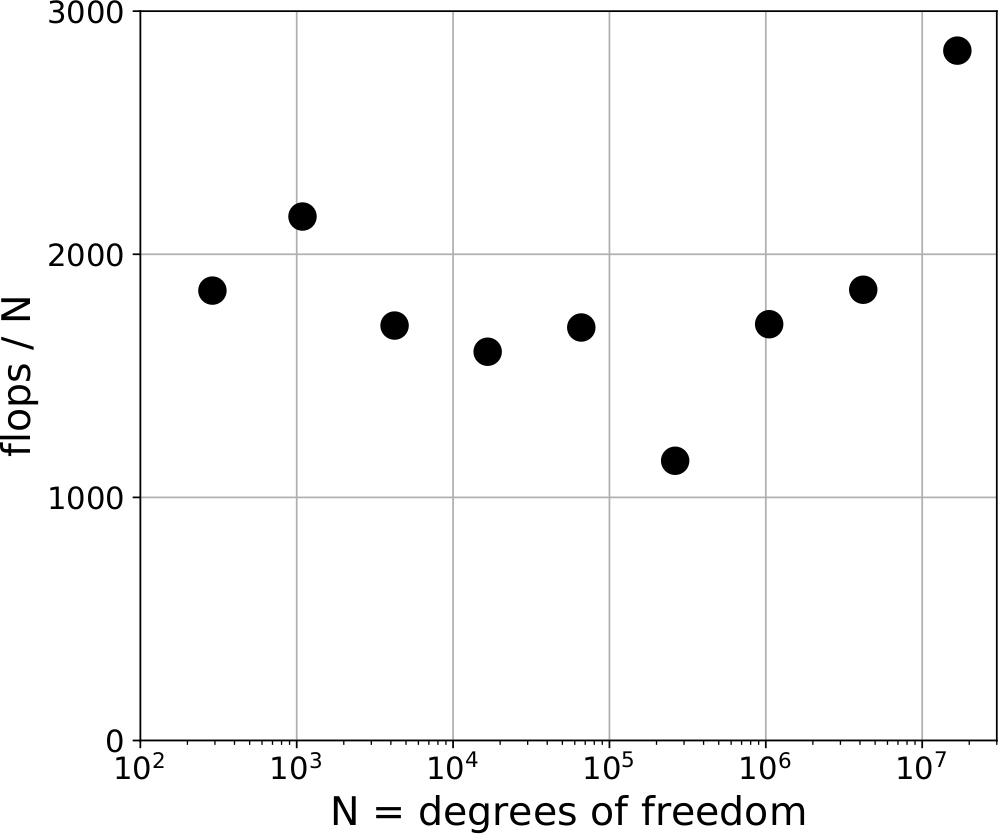
\includegraphics[width=\textwidth]{images/obstacle-flops-per-n.png}
\end{column}
\end{columns}
\end{frame}


\section{the nonlocal VI for a fluid layer in a climate}

\begin{frame}{problem: fluid layer in a climate}

\begin{center}
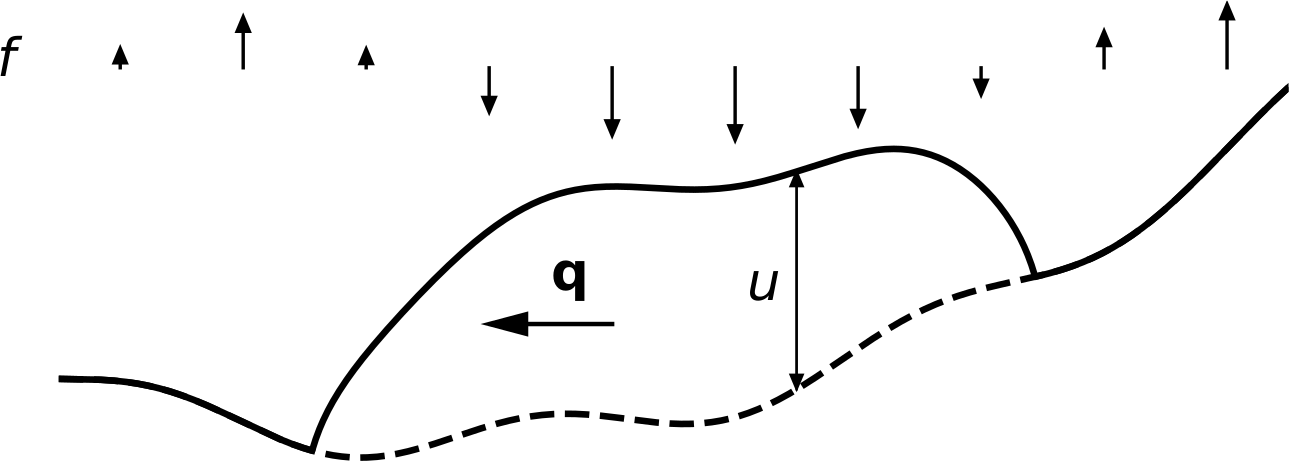
\includegraphics[width=0.6\textwidth]{images/fluid-in-climate.png}
\end{center}

\begin{itemize}
\item x
\end{itemize}
\end{frame}


\section{FAS multigrid for PDEs}

\section{a possibly scalable approach to nonlocal VIs}


\begin{frame}{the Stokes problem for ice}

\begin{itemize}
\item whether explicit or implicit, a non-shallow model solves a Stokes problem at each step:
\begin{align*}
- \nabla \cdot \left(2 \nu_\eps(D\bu)\, D\bu\right) + \nabla p - \rhoi \mathbf{g} &= \bzero && \text{in $\Lambda$} \\
\nabla \cdot \bu &= 0 && \text{''} \\
\btau_b - \bbf(\bu|_b) &= \bzero && \text{on $\Gamma_b$} \\
\bu|_b \cdot \bn_b &= 0 && \text{''} \\
\left(2 \nu_\eps(D\bu) D\bu - pI\right) \bn &= \bzero && \text{on $\Gamma_s$}
\end{align*}
\item this is the \alert{stress balance} (conservation of momentum) problem which determines velocity $\bu$ and pressure $p$
\item how fast is the numerical solution process?
    \begin{itemize}
    \item[$\circ$] how do solution algorithms \alert{scale with increasing resolution}?
    \end{itemize}
\end{itemize}
\end{frame}




\begin{frame}{multilevel NCP-coupled-to-Stokes solvers}

\begin{itemize}
\item direct attack on the problem seems to require a \alert{multilevel} solver for \alert{variational inequalities} (VIs), but in the \alert{non-local residual case}
    \begin{itemize}
    \item[$\circ$] this seems not to exist
    \item[$\circ$] the \alert{smoother} must compute an implicit-step SKE residual including surface-motion term $\Phi(s) = - \bu|_s\cdot \bn_s$ from a scalable Stokes solver
    \end{itemize}
\item near-optimal multilevel VI solvers exist for toy problems
    \begin{itemize}
    \item[$\circ$] Poisson equation obstacle problem (Brandt \& Cryer 1983; Gr\"aeser \& Kornhuber 2009)
    \end{itemize}
\item<2> \alert{help me}
\end{itemize}
\end{frame}


\section{conclusion}

\begin{frame}{\alert{summary}}

\begin{itemize}
\item x
\end{itemize}
\end{frame}


\begin{frame}{references}

{\tiny
\begin{itemize}
\item[] E.~Bueler (2021). \emph{Conservation laws for free-boundary fluid layers}, SIAM J.~Appl.~Math.~81 (5), 2007--2032, \href{https://doi.org/10.1137/20M135217X}{10.1137/20M135217X}
\item[] E.~Bueler (2021). \emph{PETSc for Partial Differential Equations}, SIAM Press, Philadelphia, PA.
\item[] E.~Bueler (2022). \emph{Performance analysis of high-resolution ice-sheet simulations}, J.~Glaciol., \href{https://doi.org/10.1017/jog.2022.113}{10.1017/jog.2022.113}
\item[] T.~Isaac, G.~Stadler, \& O.~Ghattas (2015). \emph{Solution of nonlinear Stokes equations discretized by high-order finite elements on nonconforming and anisotropic meshes, with application to ice sheet dynamics}, SIAM J.~Sci.~Comput.~37 (6), B804--B833, \href{https://doi.org/10.1137/140974407}{10.1137/140974407}
\end{itemize}
}
\end{frame}

\end{document}
